\documentclass[10pt]{article}
\usepackage[utf8]{inputenc}
\usepackage[includehead, headheight=10mm, margin=15mm ]{geometry}
\usepackage{amsmath}
\usepackage{amsthm}
\usepackage{amsfonts}
\usepackage{xcolor}
\usepackage{graphicx}
\usepackage{titling}
\usepackage{fancyhdr}
\usepackage{listings}

\title{APPM 4600 Homework 3}
\author{Edward Wawrzynek}
\date{20 September 2024}

\newcommand*{\dif}{\mathop{}\!\mathrm{d}}

\makeatletter
\def\@maketitle{%
  \newpage
  \null
  \vskip 1em%
  \begin{center}%
  \let \footnote \thanks
    {\LARGE \@title \par}%
    \vskip 1em%
    {\normalfont \@date}
  \end{center}%
  \par
  \vskip 1em}
\makeatother

\begin{document}

\pagestyle{fancy}
    \fancyhf{} % clear all header and footer fields
    \fancyhead[L]{\thetitle}
    \fancyhead[R]{\theauthor}

\makeatletter
\begin{center}
    {\Large \@title}
    \vskip 1mm
    {\normalfont \@date}
    \vskip 1em
\end{center}
\makeatother

\begin{enumerate}
    \item \begin{enumerate}
      \item We have the continuous function \(f(x) = 2x - 1 - \sin  x\). Observe that \begin{align*}
          f(0) = 2(0) -1 - \sin  0 = -1 < 0
      \end{align*} and that \begin{align*}
          f(\frac{\pi}{2}) = 2(\frac{\pi}{2}) - 1 - \sin \frac{\pi}{2} = \pi - 2 > 0.
      \end{align*} By the intermediate value theorem, \(f(x)\) has a root on the region \(x \in (0, \frac{\pi}{2})\).

      \item Observe that \(f(x)\) has derivative \begin{align*}
        f'(x) = 2 - cos(x) > 0\;\forall x \in \mathbb{R},
      \end{align*} that is, \(f\) is monotonically increasing. Thus, \(f\) has only one root on $\mathbb{R}$.

      \item The bisection code adapted from that provided in class is included below. Bisection yields an approximate root of \begin{align*}
          r \approx 0.88786221
      \end{align*}
    \end{enumerate}

    {\small \lstinputlisting[language=Python]{hw3_1.py}}

    \newpage
    \item The code used in this problem is listed below. \begin{enumerate}
      \item Bisection on \(f(x) = (x-5)^9\) finds the root \begin{align*}
          r \approx 5.00007,
      \end{align*} as expected.

      \item Bisection on the expanded form of \(f(x)\) finds the root \begin{align*}
          r \approx 5.12875,
      \end{align*} which is not within the tolerance we specified to find the root.

      \item The expanded form of \(f(x)\) undergoes catastrophic cancellation and resulting loss of precision when evaluated (we showed this on Homework 1). Thus, bisection finds a point where this loss of precision during function evaluation creates an apparent false root.
    \end{enumerate}

    {\small \lstinputlisting[language=Python]{hw3_2.py}}

    \newpage

    \item \begin{enumerate}
      \item We wish to find the roots of \(f(x) = x**3 + x - 4\) over \([1,4]\) with an absolute accuracy of \(10^-3\). From Theorem 2.1, we have that the accuracy of the \(n\)th iteration is \begin{align*}
          |p_n-p| \leq \frac{b-a}{2^n}, 
      \end{align*} so we need \begin{align*}
          n \leq \log_2 \left( \frac{b-a}{|p_n-p|} \right) = \log _2 \left( \frac{4-1}{10^-3} \right) \approx 11.5
      \end{align*} iterations to find the root to the desired accuracy. Thus, we expect no more than 11 iterations.

      \item Bisection (code below) finds the root \begin{align*}
          r \approx 1.3787
      \end{align*} after 11 iterations, which is consistent with the upper bound found in part (a).

      {\small \lstinputlisting[language=Python]{hw3_3.py}}      
    \end{enumerate}

    \newpage

    \item \begin{enumerate}
      \item We have the iterative step \(x_{n+1} = -16 + 6x_n + \frac{12}{x_n}\), \(x^* = 2\). Observe that \(f(x) = -16 + 6x + \frac{12}{x}\) has a fixed point at \(f(2) = 2\), but that \begin{align*}
          |f'(x)| = \left|6-\frac{12}{x^2}\right| > 1
      \end{align*} in the neighborhood around \(x=2\), so the iteration will not converge to \(x^* = 2\).

      \item We have the iterative step \(x_{n+1} = \frac{2}{3}x_n + \frac{1}{x_n^2}\), \(x^* = 3^\frac{1}{3}\). We have that \(x^*=3^\frac{1}{3}\) is a fixed point of the iteration and sufficient conditions for convergence (\(\left|\frac{\partial x_{n+1}}{\partial x_n}\right| < 1\) around \(x^*\)). Observe that \begin{align*}
          \lim _{n \to \infty} \frac{|x_{n+1} - x^*|}{|x_n - x^*|} = \lim _{n \to \infty} \frac{|\frac{2}{3}x_n + \frac{1}{x_n^2} - 3^\frac{1}{3}|}{|x_n - 3^\frac{1}{3}|} = \lim _{n \to \infty} \frac{|2x_n^3 -3^\frac{4}{3}x_n^2 + 3|}{|3x_n^3 - 3^\frac{4}{3}x_n^2|} = 0.
      \end{align*} Thus, the iteration converges linearly with asymptotic error constant 0.

      \item We have iterative step \(x_{n+1} = \frac{12}{1+x_n}\), \(x^* = 3\). Observe that \begin{align*}
        \lim _{n \to \infty} \frac{|x_{n+1} - x^*|}{|x_n - x^*|} = \lim _{n \to \infty} \frac{\left|\frac{12}{1+x_n} - 3\right|}{\left|x_n - 3\right|} = \lim _{n \to \infty} \frac{\left|\frac{12-3-3x_n}{1+x_n}\right|}{\left|x_n - 3\right|} = \lim _{n \to \infty} \left| 3\frac{3-x_n}{(x_n + 1)(x_n - 3)} \right| = \frac{3}{4}.
      \end{align*} Thus, the iteration converges linearly with asymptotic error constant \(\frac{3}{4}\).
    \end{enumerate}

    \newpage
    \item The code for this question is listed below. \begin{enumerate}
      \item A plot of \(f(x) = x - 4\sin(2x) - 3\) is shown below. The function has five roots.
      
      \begin{center}
        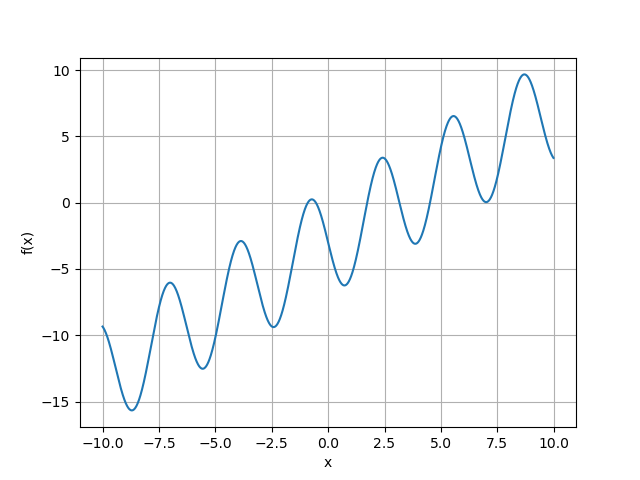
\includegraphics[width=0.5\textwidth]{hw3_5_a.png}
      \end{center}

      \item Fixed point iteration of \begin{align*}
          x_{n+1} = -\sin  (2x_n) + \frac{5}{4}x_n - \frac{3}{4}
      \end{align*} gives only the roots \begin{align*}
          r_1 &\approx -0.544442400, \\
          r_2 &\approx 3.161826486.
      \end{align*} These are the only roots that occur where \begin{align*}
          \left|\frac{\partial x_{n+1}}{\partial x_n}\right| = \left| -2\cos(2 x_n) + \frac{5}{4} \right| \leq 1,
      \end{align*} which is the only region over which we can expect the fixed point iteration to converge.
    \end{enumerate}

    {\small \lstinputlisting[language=Python]{hw3_5.py}}   

\end{enumerate}


\end{document}